\chapter{Spell Weavers}




\begin{table*}[ht!]
\begin{small}
\rowcolors{2}{}{commentgreen}
\begin{center}
\begin{tabular}{ccccllllll}
\multicolumn{5}{l}{\parbox[l][0.6cm][c]{8cm}{\textbf{The Trickster}}} & 
\multicolumn{5}{c}{\textbf{-- Spell Slots --}}
\\
\hline 
\textbf{Level} & \textbf{Prof} & \textbf{Mana} & \textbf{Points} & \parbox[l][0.6cm][c]{8cm}{\textbf{Features}} & \textbf{1st} & \textbf{2nd} & \textbf{3rd} & \textbf{4th} & \textbf{5th}
\\ 
1st & +2 & 1d6 & 2 & \parbox[l][0.6cm][c]{8cm}{Mend, Path feature} & 2 & - & - & - & -
\\
2nd & +2 & 1d6 & 3 & \parbox[l][0.6cm][c]{8cm}{Extra feat} & 3 & - & - & - & -
\\
3rd & +2 & 1d6 & 3 & \parbox[l][0.6cm][c]{8cm}{Path feature} & 4 & 2 & -& - & -
\\
4th & +2 & 1d8 & 3 & \parbox[l][0.6cm][c]{8cm}{Extra feat, Ability Score Improvement} & 4 & 3 & - & - & -
\\
5th & +3 & 1d8 & 4 & \parbox[l][0.6cm][c]{8cm}{Weave Ward} & 4 & 3 & 2 & - & -
\\
6th & +3 & 1d8 & 4 & \parbox[l][0.6cm][c]{8cm}{Extra feat} & 4 & 3 & 3 & - & -
\\
7th & +3 & 1d8 & 5 & \parbox[l][0.6cm][c]{8cm}{Path feature} & 4 & 3 & 3 & 1 & -
\\
8th & +3 & 1d8 & 5 & \parbox[l][0.6cm][c]{8cm}{Extra feat, Ability Score Improvement} & 4 & 3 & 3 & 2 & -
\\
9th & +4 & 1d10 & 6 & \parbox[l][0.6cm][c]{8cm}{Path feature} & 4 & 3 & 3 & 3 & 1 
\\
10th & +4 & 1d10 & 6 & \parbox[l][0.6cm][c]{8cm}{Extra feat} & 4 & 3 & 3 & 3 & 2 
\\

\hline
\end{tabular}
\end{center}
\end{small}
\end{table*}


\begin{multicols*}{2}

\section*{Class Features} 

As a spell-weaver, you gain the following class features.

\textbf{Hit Dice:} 1d6

\textbf{Hit Points at 1st Level:} 10 + your Constitution modifier

\textbf{Hit Points at Higher Levels:} 2 + your Constitution modifier per fighter level after 1st


\textbf{Armor:} None

\textbf{Weapons:} Daggers, darts, slings, quarterstaffs, light crossbows, javelins, clubs, and spears

\textbf{Saving Throws:} Wisdom, Charisma

\textbf{Skills:} Choose three from Arcana, Animal Handling, Insight, Medicine, History, Investigation, Nature, Perception, Religion, and Persuasion
    
\section*{Mana} 

You have a pool of mana dices to use. Spell-weavers use mana to bend reality. Novice spell-weavers use mana to mend wounds while seasoned ones apply powerful metamagic to their spells.



\begin{itemize}
    \item You regain all mana points when finish a long rest.
    \item You can sacrifice part of your life force to regain mana points. Roll your Hit dice you regain 1 mana point or 2 in case you roll a 5 or 6.
\end{itemize}


    
\section*{Mend} 

As a bonus action, you can spend one mana point and a creature of your choice that you can see within 60 feet of you regains Hit Points equal to your mana die + your Spellcasting Ability modifier.



\section*{Spellcasting}

You have learned to untangle and reshape the fabric of reality through sheer force of will.

\textbf{Cantrips}

You learn three cantrips draw from the cleric, wizard, or druid spell list. 


\textbf{Spells Known of 1st Level and Higher}

You know three 1st-level spells of your choice.

The Spell-weaver Spellcasting table shows how many spell slots you have to cast your spells of 1st level and higher. To cast one of these spells, you must expend a slot of the spell's level or higher. You regain all expended spell slots when you finish a long rest.


Whenever you gain a level in this class, you learn two new spells. Additionally, you can replace one of the spells you know with another spell of your choice from the trickster spell list. The new spell must be of a level for which you have spell slots.

As per your GM discretion, you can learn spells through other means. For example, an arcanist can scribe scrolls, a druid might join a ritual in an ancient glade and be bestowed with new powers, while a cleric can learn new spells from their gods' blessing.
Please remember that it's up to you and your GM do reach consensus on when it's appropriate to learn spells in this exceptional way.

\textbf{Spellcasting Ability}

Intelligence or Wisdom is your spellcasting ability for your spells. You use your Intelligence or Wisdom whenever a spell refers to your spellcasting ability. In addition, you use your Intelligence or Wisdom modifier when setting the saving throw DC for a spell you cast and when making an attack roll with one.

\textbf{Spell save DC} = 8 + your proficiency bonus + your Intelligence/Wisdom modifier

\textbf{Spell attack modifier} = your proficiency bonus + your Intelligence/Wisdom modifier


\section*{Weave Ward}

You weave arcane energy to create a protective ward that boost the party's morale.

Starting at 5th level, whenever you or a friendly creature within 20 feet of you must make a saving throw, the creature gains a bonus to the saving throw equal to your proficiency bonus. You must be conscious to grant this bonus.


\begin{Figure}
\centering

\includegraphics[width=\textwidth]{img/mender.png}
{\scriptsize Art by Larry Elmore}
\end{Figure}



    
\end{multicols*}

\clearpage


\begin{multicols*}{2}

\section{Arcanist}

\subsection*{Arcane Shield}

Twice per combat, when you are hit by an attack or targeted by the magic missile spell, you can spend your reaction to create an invisible barrier of magical force appears and protects you. Until the start of your next turn, you have a +5 bonus to AC, including against the triggering attack, and you take no damage from magic missile.

Additional uses of this class feature require spending mana points.

\subsection*{Metamagic}

At 3rd level, you gain the ability to twist your spells to suit your needs. Refer to the arcanists's matamagic table for details.

The more powerful the metamagic, the more instability there is in successfully applying it to a spell. For example, there is always a risk that you won't sculpt a spell to protect all your allies.

You can use only one Metamagic option on a spell when you cast it, unless otherwise noted.

\begin{Figure}
\centering
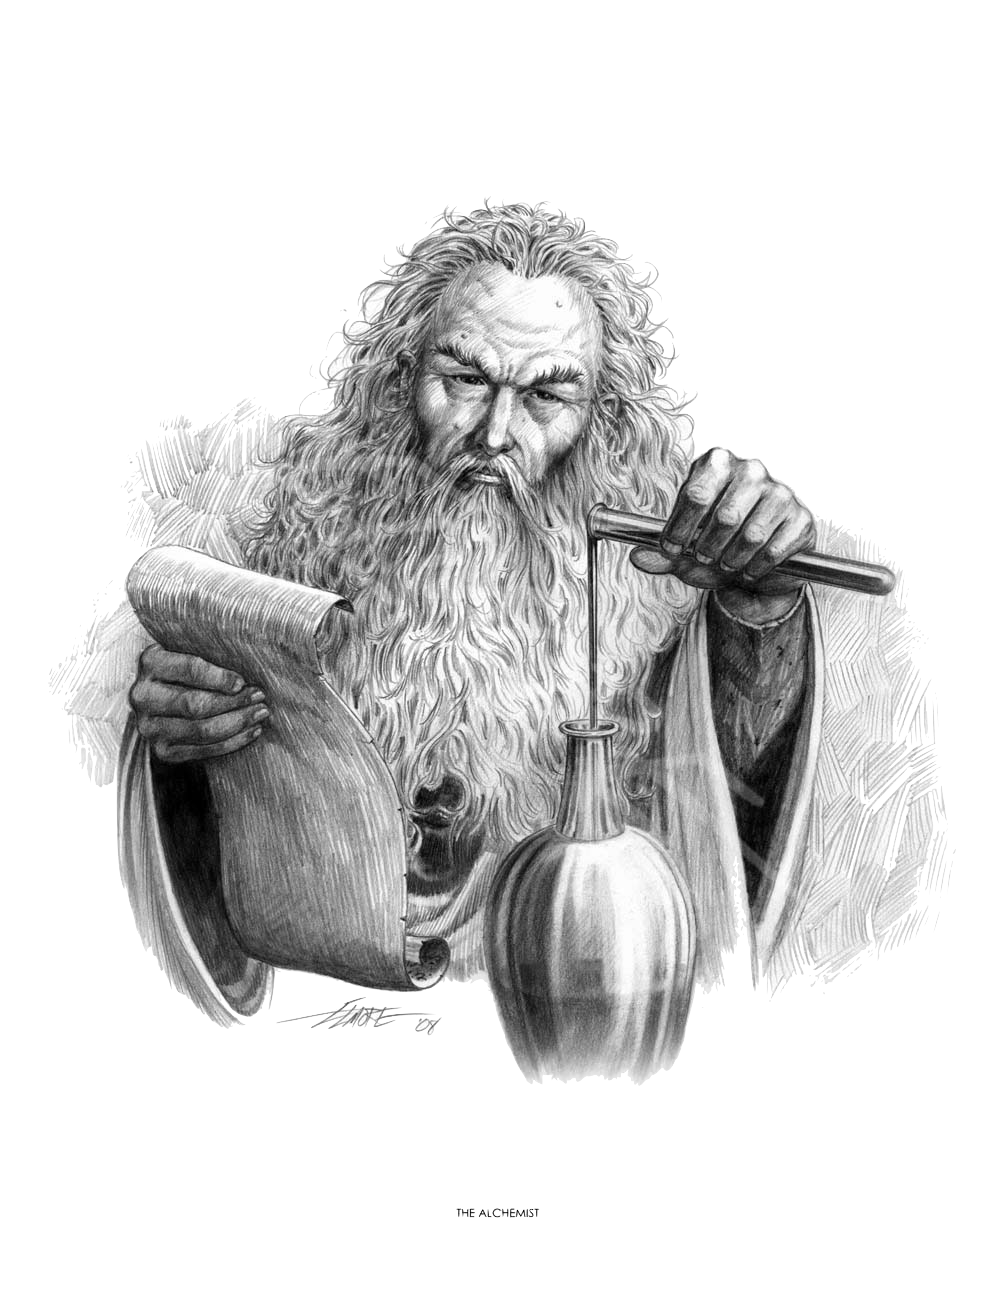
\includegraphics[width=\textwidth]{img/wizard.png}
\end{Figure}

\subsection*{Dispel Weave}

At 5th level, you can suppress any harmful spell effects on a creature or in an area of 20 feet around you. Spend one mana point and roll your mana die, harmful effects are suppressed by your mana die minutes. This class feature requires concentration.

\subsection*{High Weave}

At 9th level, you have achieved such mastery over certain spells that you can cast them at will. Choose two 1st-level arcanist spels. You can cast those spells at their lowest level without expending a spell slot. If you want to cast either spell at a higher level, you must expend a spell slot as normal.

Additionally, apply one of the following effects to your high weave spells:

\header{High Weave Effects}
\begin{rpg-table}
   	Deadly  & Add your mana die as extra damage to one creature hit by the spell.  \\
   	Warding  & A spell that requires concentration or that has a fixed duration (e.g., Mage Armor) and that targets you or an ally grants temporary hit points equal to your mana die \\
    Execrate  & The first time a creature succeeds on a save against your spell, roll your mana die. On a 1, the creature fails. This effect applies only once per spell. \\
\end{rpg-table}



\medskip

\textbf{Named Spell:} Add your name as a suffix or prefix to your high weave spells. For example, if Maya has choose 
magic missle as her high weave, people around the world might start to recognize it as Maya's magic missile. 


\textbf{Cosmetic Changes:} Discuss with your DM any cosmetic changes that distinguish your high weave spells from mudane ones, e.g., Maya's magic missiles are three green darts always floating around her head like a corona. At her command, the darts fly towards a target and a few second after, new darts appear.

    
\end{multicols*}


\clearpage

\begin{table}[ht!]
\begin{small}
\rowcolors{2}{}{commentgreen}
\begin{center}
\begin{tabular}{ll}
\multicolumn{2}{l}{\parbox[l][0.6cm][c]{15cm}{\textbf{Arcanist Metamagic}}} 
\\
\hline 
\textbf{Name} & \parbox[l][0.6cm][c]{15cm}{\textbf{Description}}
\\ 
Sculpt Spells & \parbox[l][2.8cm][c]{15cm}{
When you cast a spell that forces other creatures to make a saving throw, you can protect some of those creatures from the spell’s full force. To do so, you spend 1 mana point and choose a number of those creatures up to your mana die (minimum of one creature). The chosen creatures automatically succeed on their saving throws against the spell, and they take no damage if they would normally take half damage on a successful save.
}
\\ 
Distant Spell & \parbox[l][2.2cm][c]{15cm}{
When you cast a spell that has a range of 5 feet or greater, you can spend 1 mana point to double the range of the spell.
\\
When you cast a spell that has a range of touch, you can spend 1 mana point to make the range of the spell 30 feet.
}
\\ 
Empowered Spell & \parbox[l][2.8cm][c]{15cm}{
When you roll damage for a spell, you can spend 1 mana point to reroll a number of the damage dice up to your spellcasting modifier (minimum of one). You must use the new rolls. Additionally, you add one mana die to the damage of the spell.
\\
You can use Empowered Spell even if you have already used a different Metamagic option during the casting of the spell.
}
\\
Heightened Spell & \parbox[l][1.6cm][c]{15cm}{
When you cast a spell that forces a creature to make a saving throw to resist its effects, you can spend 2 mana points to give one target of the spell a penality to its saving throw equals to your mana die on its first saving throw made against the spell.
}
\\
Quickened Spell & \parbox[l][1.6cm][c]{15cm}{
When you cast a spell that has a casting time of 1 action, you can spend 2 mana points to change the casting time to 1 bonus action for this casting.
}
\\
\hline
\end{tabular}
\end{center}
\end{small}
\end{table}    


\begin{multicols*}{2}
\begin{Figure}
\centering
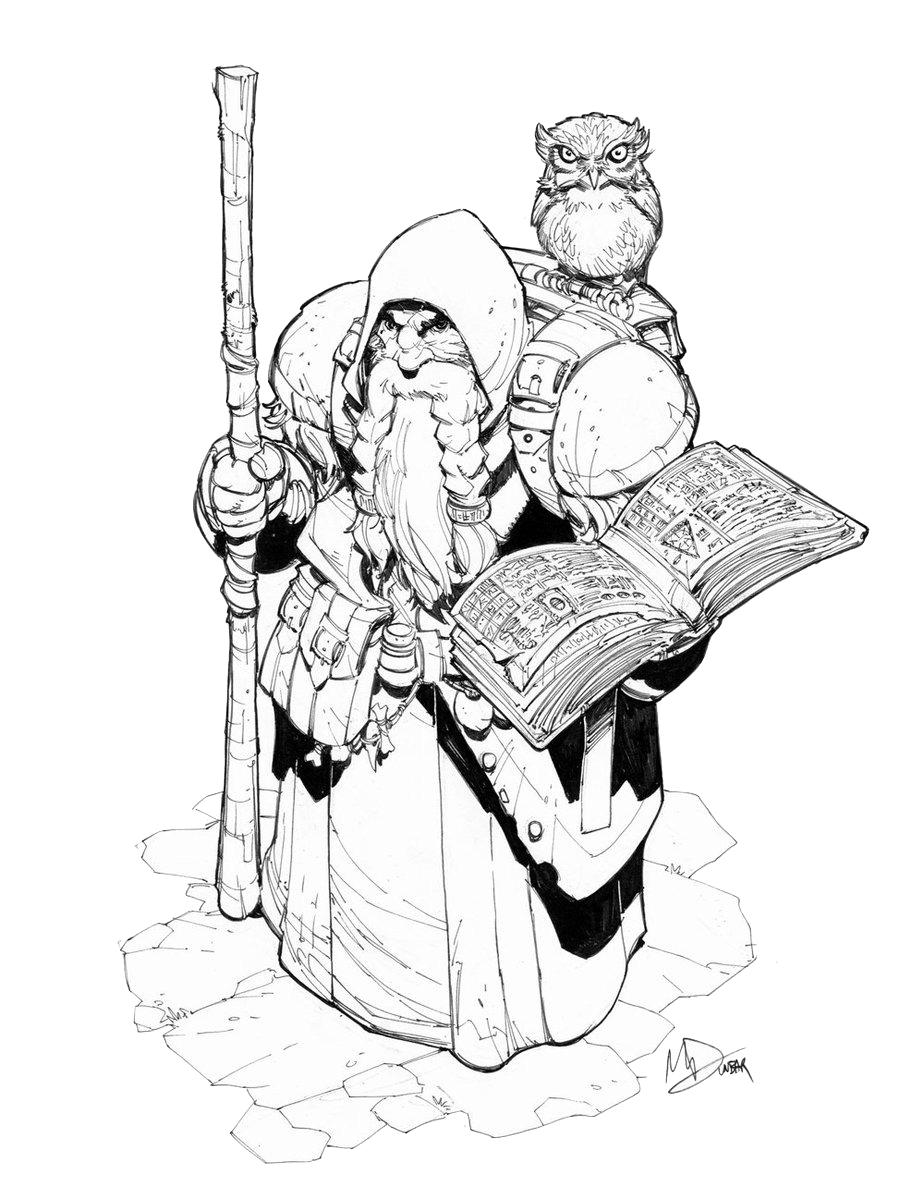
\includegraphics[width=\textwidth]{img/wizard-2.png}
\end{Figure}
    
\end{multicols*}

    


\begin{multicols*}{2}

\section{Elementalist}

\subsection*{Bend Elements}

Twice per combat, when you or a creature within 30 feet of you takes acid, cold, fire, lightning, or thunder damage, you can use your reaction to grant resistance to the creature against that instance of the damage.

Additional uses of this class feature require spending mana points.

\subsection*{Shaman Training}

You gain proficiency with light armor and shields.

\subsection*{Wild Magic}

At 3rd level, you gain the ability to tap into the raw energy of the primordials. Refer to the Elementalist's wild magic table for details.

If your wild magic requires you to place a totem, treat it as a small creature that appears in an unoccupied space on a horizontal surface within 5 feet of you.

The totem has an AC of 18 and a number of hit points equal to 4 times your level. It is immune to poison damage, psychic damage, and all conditions. If it is forced to make an ability check or saving throw, treat all it's ability scores as 10 (+0). 

On each of your turns, you can take a bonus action to cause the totem to activate if you are within 60 feet of it. As part of the same bonus action, you can direct the totem to slowly fly up to 15 feet to an unoccupied space near the ground. While the totem has fly speed, it hovers just above the ground.


\subsection*{Armor of Hera}

% A protective magical force surrounds you, manifesting as a spectral frost or cinder that covers you and your gear.
% After a short rest, you gain 10 temporary hit points. While you have these hit points, a creature that hits you with a melee attack takes 5 cold or fire damage. You choose the damage type when you gain these temporary hit points.

\subsection*{Storm, Earth, and Fire}

\begin{Figure}
\centering
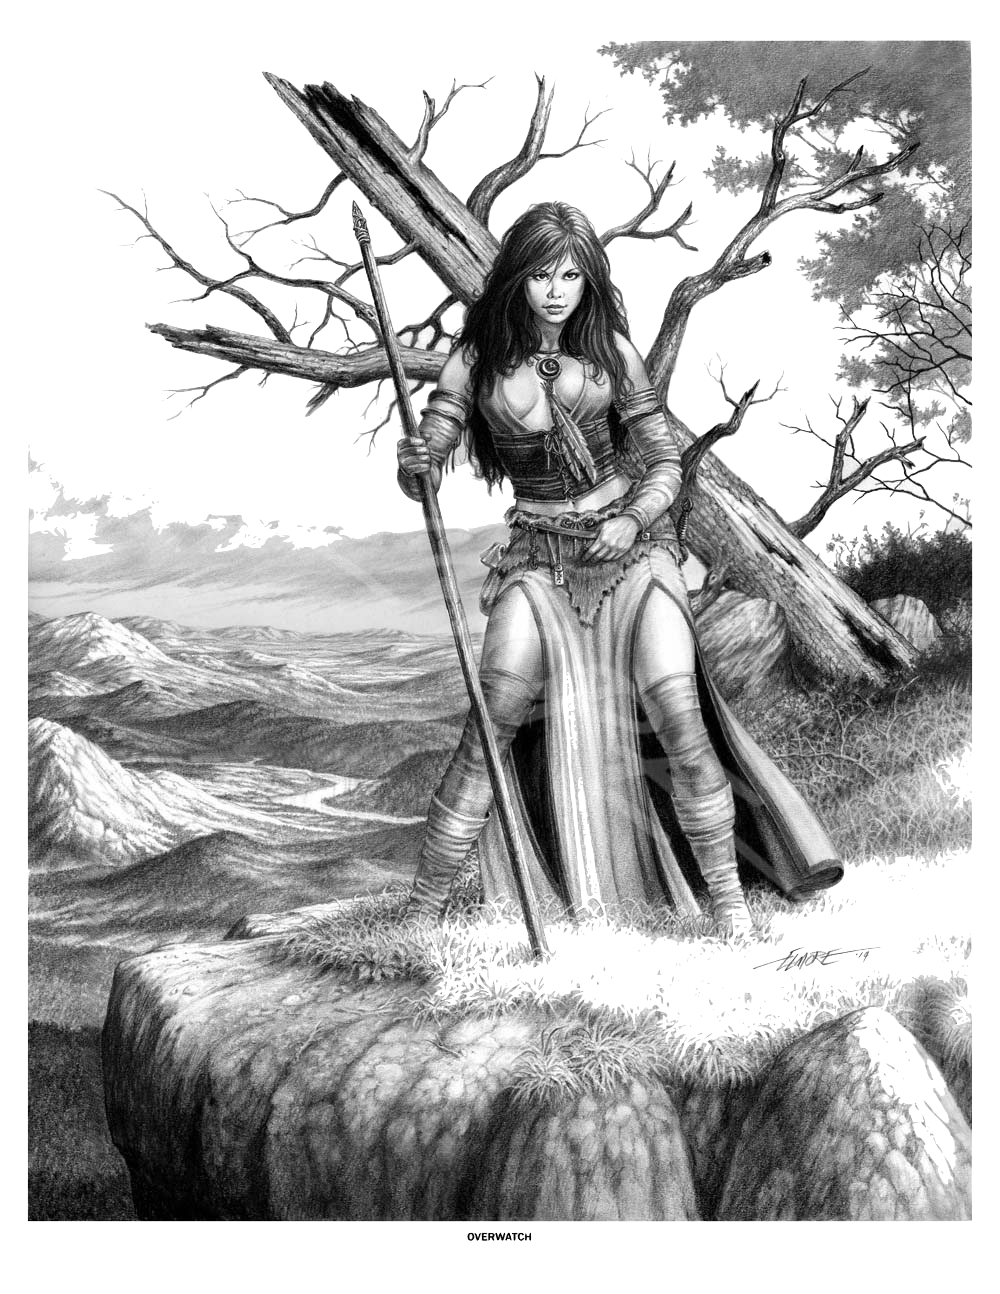
\includegraphics[width=\textwidth]{img/druid-2.png}
\end{Figure}
    
\end{multicols*}


\clearpage

\begin{table}[ht!]
\begin{small}
\rowcolors{2}{}{commentgreen}
\begin{center}
\begin{tabular}{ll}
\multicolumn{2}{l}{\parbox[l][0.6cm][c]{15cm}{\textbf{Arcanist Metamagic}}} 
\\
\hline 
\textbf{Name} & \parbox[l][0.6cm][c]{15cm}{\textbf{Description}}
\\ 
Air & \parbox[l][2.8cm][c]{15cm}{
You can spend one mana point to create an almost invisible sphere of wind and hovering leaves. The totem emits strong winds causing disadvantage in the first ranged attacks against a creature within 10 feet of the totem. Including itself. This effect activates only once per creature per round.
\\
This totem can fly in any direction. 
}
\\ 
Earth & \parbox[l][2cm][c]{15cm}{
You can spend one mana point to create an orb of dust, rocks, and gravel as a bonus action. The totem emits a burst of positive energy that grants itself and up to three creatures of your choice within 10 feet of it a number of temporary hit points equal to you mana die. The dust barrier protects the creature from natural heat.
}
\\
Fire & \parbox[l][2cm][c]{15cm}{
You can spend one mana point to create a sphere of flames and cinder. The totem must hover directly 5 feet above a create. The warm flames protect the creature from natural cold. Once per round, whenever the protected creature takes melee damage, the sphere rebukes with flames. The attacking creature takes your mana die fire damage.
}
\\ 
Water & \parbox[l][2.2cm][c]{15cm}{
You can spend one mana point to create an orb of water and ice. The water sphere fires ice javelins upon your command. 
Make a ranged spell attack, originating from the water sphere, at one creature or object within 120 feet of it. On a hit, the target takes your mana die damage + your spellcasting ability modifier ice damage.
}
\\
\hline
\end{tabular}
\end{center}
\end{small}
\end{table}    


\begin{multicols*}{2}
\begin{Figure}
\centering

\includegraphics[width=\textwidth]{img/bard.png}
\end{Figure}
    
\end{multicols*}

        


\begin{multicols*}{2}

\section{Cleric}

\subsection*{Healing Hands}

\subsection*{Sacred Immolation}

\subsection*{Divine Smite}

\subsection*{Aura of Courage}

\begin{Figure}
\centering
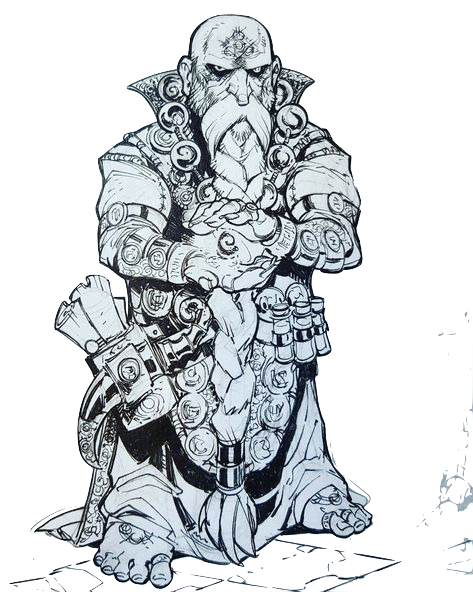
\includegraphics[width=\textwidth]{img/cleric.png}
\end{Figure}
    
\end{multicols*}

    
    